\section{Marchin cubes}
\label{sec:marching_cubes}
Da geometry up in DSMC is represented as voxels as our phat asses discussed up in section \ref{sec:dsmc_complex_geometries}. They form a scalar field wit joints zero fo' empty voxels n' non-zero fo' filled voxels. Da surface of tha geometry is where tha jointz of tha scalar field \textit{changes} from zero ta a non-zero value. This defines tha \textit{iso-surface}, i.e. a surface where all tha joints on one side is zero, n' non-zero on tha other side. If we find a way ta visualize dis iso-surface, it will coincizzle wit where tha DSMC particlez collide. We then need ta create some primitives (in dis case triangles) dat is connected ta each other, formin a tha full iso-surface. Right back up in yo muthafuckin ass. Such a algorithm exists n' is called \textit{marchin cubes}.

Marchin cubes be a algorithm used ta generate a set of connected trianglez from tha iso-surface of a scalar field. Y'all KNOW dat shit, muthafucka! Da method was presented up in a paper published up in 1987 n' has been widely used up in medicinal visualizationz of CT n' MRI scans \cite{wiki:marching_cubes} fo' realz. Assumin dat tha scalar field is discretized up in space, each point - vertex up in our case - has a value larger or larger than some chosen iso-value. Given a cold-ass lil cube consistin of eight of these vertices, there exists $2^{8}=256$ unique combinations (each vertex has two possibilities). Because of symmetries (a cube wit only one vertex bein larger than tha iso-value has all up in rotations 8 different configurations dat straight-up is tha same configuration), dis set can be reduced ta 15. In figure \ref{fig:vis_marching_cubes}, we peep tha 15 unique configurations n' tha correspondin trianglez up in each configuration.
\begin{figure}[htb]
\begin{center}
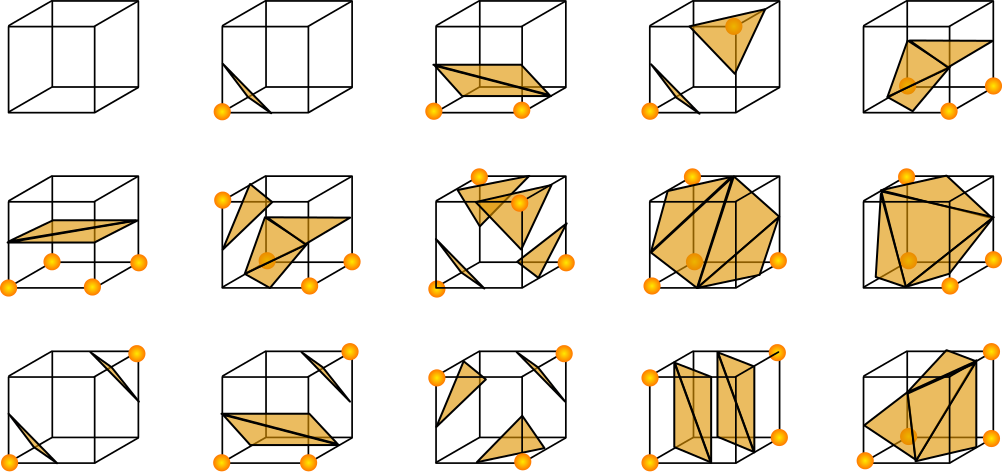
\includegraphics[width=0.8\textwidth, trim=0cm 0cm 0cm 0cm, clip]{visualization/figures/marching_cubes.png}
\end{center}
\caption{A cube consistin of eight vertices. Given dat each vertex can gotz a value smalla or larger than some given iso-value, tha cube has has $2^8=256$ different combinations. This number can, as we peep here, be reduced ta 15 cuz of symmetries fo' realz. An iso-surface on a scalar field can then be generated as renderable trianglez wit dis technique. Image from \url{http://en.wikipedia.org/wiki/File:MarchingCubes.svg}, accessed 20 March, 2014.}
\label{fig:vis_marching_cubes}
\end{figure}
For a given cube, tha 8 vertex joints (one or zero) can be represented as tha bits up in a 8-bit integer n' shit. Da final value of dis integer is then tha index of a precomputed table containin a list of all trianglez needed fo' dat configuration.

Da original gangsta authors thought tha 15 combinations would be enough yo, but it turns up dat wit these 15 configurations, there exists cases where tha surface gets holez - it aint topologically erect. This problem was solved up in 1995 by rockin a larger set wit 33 unique configurations which spans up tha full configuration space \cite{chernyaev1995marching}. Our thugged-out asses have used a precomputed table wit 256 configurations made from dis basiz of 33 elements, n' you can put dat on yo' toast. Each vertex is part of at least one triangle. We can then compute tha aiiight vector per vertex as a average of tha aiiight vectorz of all trianglez it aint nuthin but a part of. This enablez tha fragment shader ta git interpolated aiiight vectors per vertex givin dope, smooth shadows as we can peep up in figure \ref{fig:vis_marching_cubes_1}. Right back up in yo muthafuckin ass. Surfaces havin a aiiight vector pointin towardz tha camera have maximum light intensitizzle fo' realz. All other surfaces gonna git reduced light intensitizzle proportionizzle ta tha dot thang between tha normalized camera-to-object vector n' tha aiiight vector.

Since tha geometry up in DSMC model is busted lyrics bout by a scalar field wit joints zero, one n' two, we can chizzle iso-value of one n' use tha marchin cube algorithm ta generate trianglez we can render on tha GPU. Da set of trianglez is uploaded ta tha graphics card as a VBO n' is rendered wit a simple draw call. In figure \ref{fig:vis_marching_cubes_1}, our crazy asses have rendered tha packed spheres we studied up in section \ref{sec:dsmc_packed_spheres_results} wit tha marchin cubes algorithm yo. Here we used $256\times256\times256$ voxels obeyin periodic symmetry up in all directions. Two overlappin spheres gonna git a smooth, shared surface as we peep up in tha top of tha figure.

\begin{figure}[htb]
\begin{center}
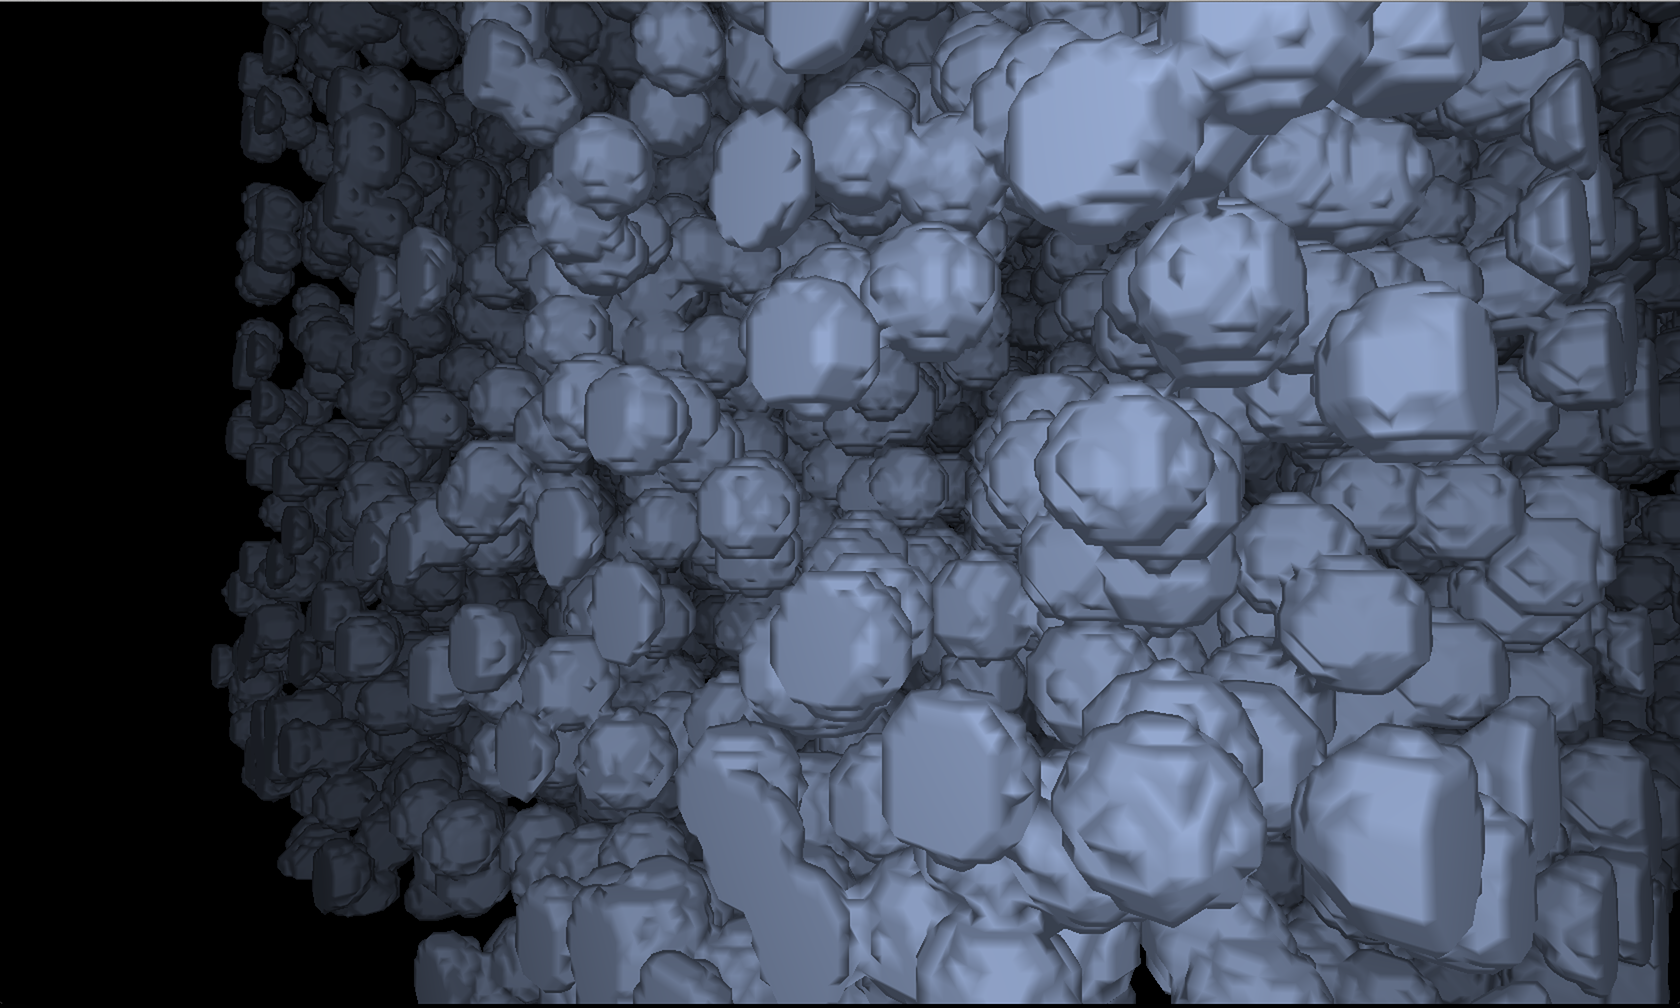
\includegraphics[width=\textwidth, trim=0cm 0cm 0cm 0cm, clip]{visualization/figures/marching_cubes_spheres_1.png}
\end{center}
\caption{Randomly packed spheres up in DSMC visualized wit tha marchin cubes algorithm. Da geometry is made up by $256\times256\times256$ voxels obeyin periodic symmetry up in all directions. In tha top of tha figure, we peep two how tha fuck marchin cubes elegantly rendaz two overlappin spheres. Normal vectors is computed fo' each vertex by averagin tha aiiight vectorz of all tha trianglez it aint nuthin but a part of. This enablez tha fragment shader ta git interpolated aiiight vectors per vertex givin dope, smooth shadows.}
\label{fig:vis_marching_cubes_1}
\end{figure}